\documentclass[10pt]{beamer}
\mode<presentation>
{
\usetheme{Darmstadt}      % or try Darmstadt, Madrid, Warsaw, ...
\usecolortheme{default} % or try albatross, beaver, crane, ...
\usefonttheme{default}  % or try serif, structurebold, ...
\setbeamertemplate{navigation symbols}{}
\setbeamertemplate{caption}[numbered]
\setbeamersize{text margin left=10pt,text margin right=10pt}
}

\usepackage[english]{babel}
\usepackage[utf8x]{inputenc}
\usepackage{graphicx}
\graphicspath{ {./pictures/} }

\title[Kvam Presentation 1]{Civil Violence : The impact of Social Media}
\author{Daniël Vink, Floris de Vries, Roman Peerboom, Sam Kuilboer, Viviane Desgrange}
\institute{University of Amsterdam}
\date{\today}

\begin{document}

    \begin{frame}
        \titlepage
    \end{frame}

% Uncomment these lines for an automatically generated outline.
%\begin{frame}{Outline}
%  \tableofcontents
%\end{frame}

    \begin{frame}{Overview}
        \tableofcontents
    \end{frame}

    \section{Introduction}

    \begin{frame}{Civil violence model [Epstein 2002]}

        \begin{itemize}
            \item A central authority attempts to suppress civil violence among population
            \item Agents are civilians or law enforcement officers
        \end{itemize}

        \hfill
        \hfill

        \begin{columns}
            \begin{column}{.6\textwidth}
                \textbf{Civilian agents}:
                \begin{itemize}
                    \item Grievance G = Hardship $\times$ (1 - Legitimacy)
                    \item Net Risk N = Arrest Probability $\times$ Risk Aversion
                    \item Became active when G - N $>$ T
                    \item Move randomly in neighbouring area
                \end{itemize}
            \end{column}
            \begin{column}{.4\textwidth}
                \textbf{Cop agents}:
                \begin{itemize}
                    \item Move randomly if no active agent
                    \item Arrest neighbouring active agent
                    \item Never defect the revolution
                \end{itemize}
            \end{column}
        \end{columns}

% \begin{minipage}[t]{0.56\linewidth}

% \end{minipage}
% \hfill
% \begin{minipage}[t]{0.40\linewidth}

%  \end{minipage}

    \end{frame}

    \begin{frame}{Problem studied : the impact of social media}

        \begin{itemize}
            \item Epstein model did not consider social bond between agents
            \item Emergence of social networks in the 2000s brings new dynamics to civil violence
            \item Recent literature cover influence of social media on civil violence without focus on network topology or influencer agent
        \end{itemize}

        \hfill

        \textbf{Interrogations our research attempt to answer}:
        \begin{itemize}
            \item How network topologies influence the civil violence model ?
            \item What is the role of well-connected individuals in spread of social violence ?
            \item Can civil violence be handled by control of influencer agents ?
        \end{itemize}

    \end{frame}

    \section{Extension of civil violence model}

    \begin{frame}{How ? Contagious Hardship}

        Individual hardship H is influenced by hardship of other agents

        \begin{equation}
            H(i,t) = H_{endo}(i) + H_{contg}(i,t)
        \end{equation}

        \begin{itemize}
            \item $H_{endo}$ is the individual hardship draw from $U(0, 1)$
            \item $H_{contg}$ is hardship received from other agents
        \end{itemize}

        \begin{equation}
            H_{contg}(i,t) =H_{contg}(i,t - \delta t) + \sum\limits_{j = 1}^{N_{ir, A}} h_{ij}
        \end{equation}

        Every time step, received hardship is added to contagious hardship


    \end{frame}

    \begin{frame}{How ? Feedback legitimacy}

        Making legitimacy dependent on the actions of the government

        Legitimacy is calculated every time step

        \begin{equation}
            L_B(t) = L_0 \times (1- \sum\limits_{i = 1}^{m} \beta^i_i)
        \end{equation}

        \begin{equation}
            \beta_i = \frac{Amount\ of\ agents\ put\ in\ jail\ in\ period\ i}{Amount\ of\ agents\ not\ in\ jail\ at\ the\ start\ of\ period\ i}
        \end{equation}

    \end{frame}

    \begin{frame}{How ? Social Networks layer}

        Imitating social media by connecting agents from all over the grid

        \begin{columns}

            \begin{column}{0.3\textwidth}
                \begin{figure}
                    \centering
                    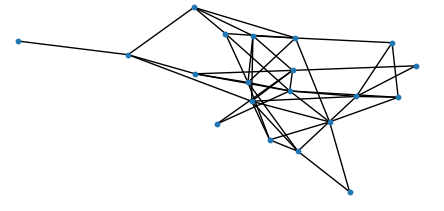
\includegraphics[width=\textwidth]{pictures/networks/ernos_renyi.png}
                    \caption{Ernos Renyi}
                \end{figure}
            \end{column}
            \begin{column}{0.3\textwidth}
                \begin{figure}
                    \centering
                    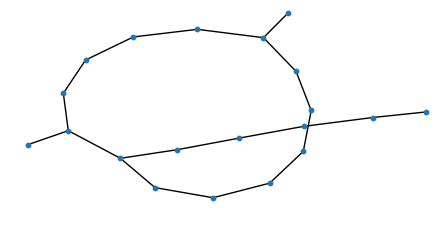
\includegraphics[width=\textwidth]{pictures/networks/watts_strogatz.png}
                    \caption{Watts-Strogatz}
                \end{figure}
            \end{column}
            \begin{column}{0.3\textwidth}
                \begin{figure}
                    \centering
                    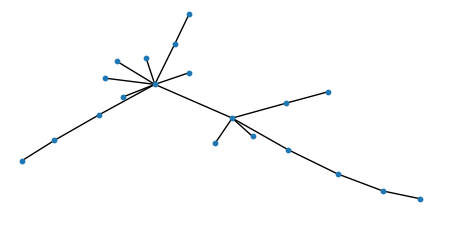
\includegraphics[width=\textwidth]{pictures/networks/barabasi_albert.png}
                    \caption{Barabasi-albert}
                \end{figure}
            \end{column}
        \end{columns}

    \end{frame}

    \begin{frame}{How ? Influencers hub}

        If the civilian agent node degree is greater than a threshold : he is an \textbf{influencer}

        \begin{figure}
            \centering
            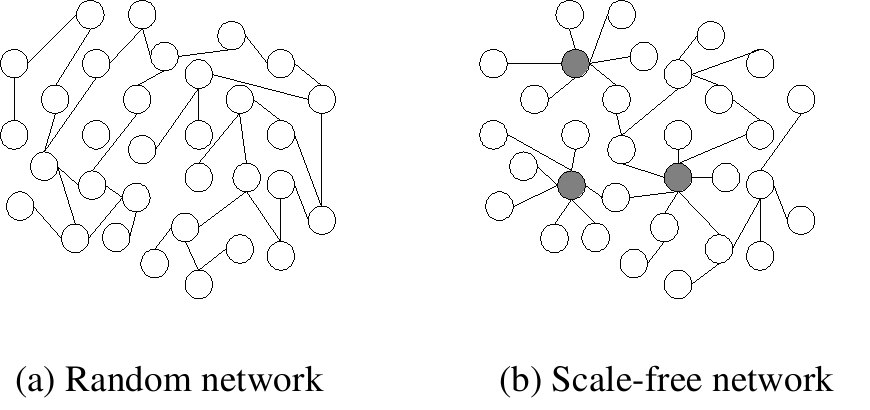
\includegraphics[width=.75\textwidth]{pictures/networks/influencer_network.jpg}
        \end{figure}

    \end{frame}


    \begin{frame}{Demonstration}

        \begin{columns}
            \begin{column}{.3\textwidth}
                \begin{figure}
                    \centering
                    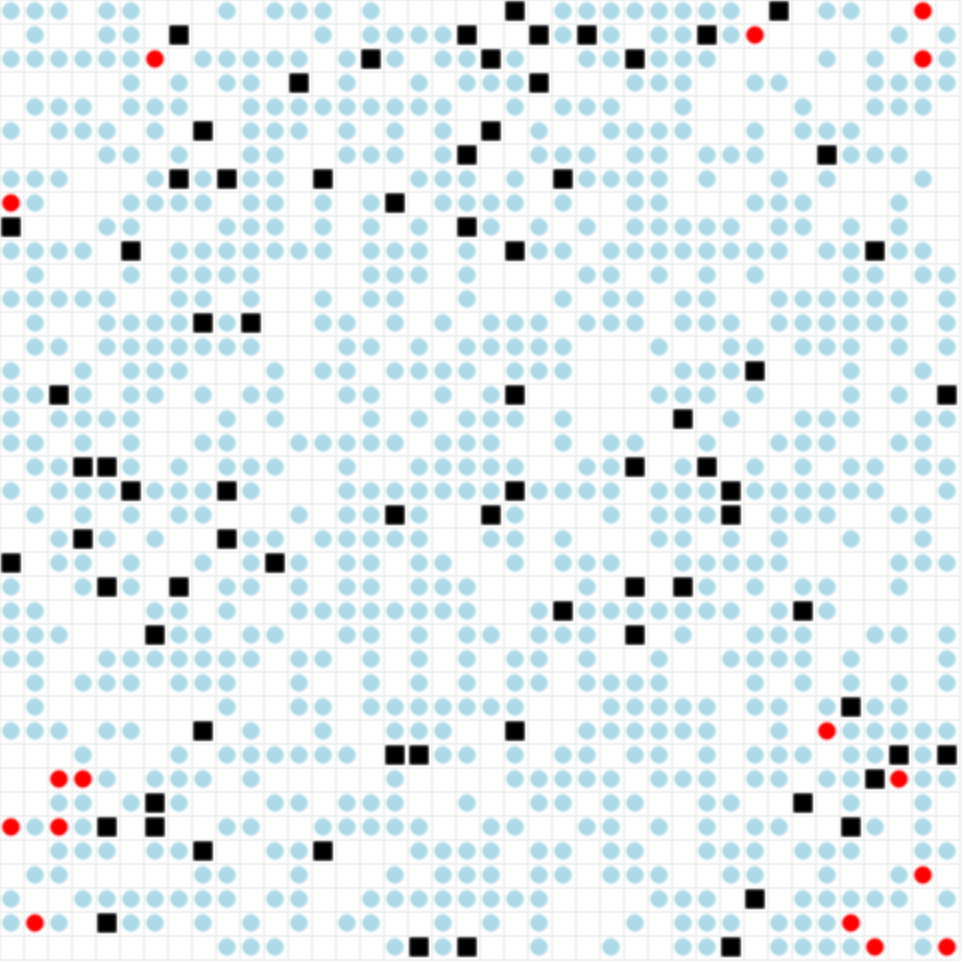
\includegraphics[width=.9\textwidth]{pictures/demonstration/spread_1.png}
                \end{figure}
            \end{column}
            \begin{column}{.3\textwidth}
                \begin{figure}
                    \centering
                    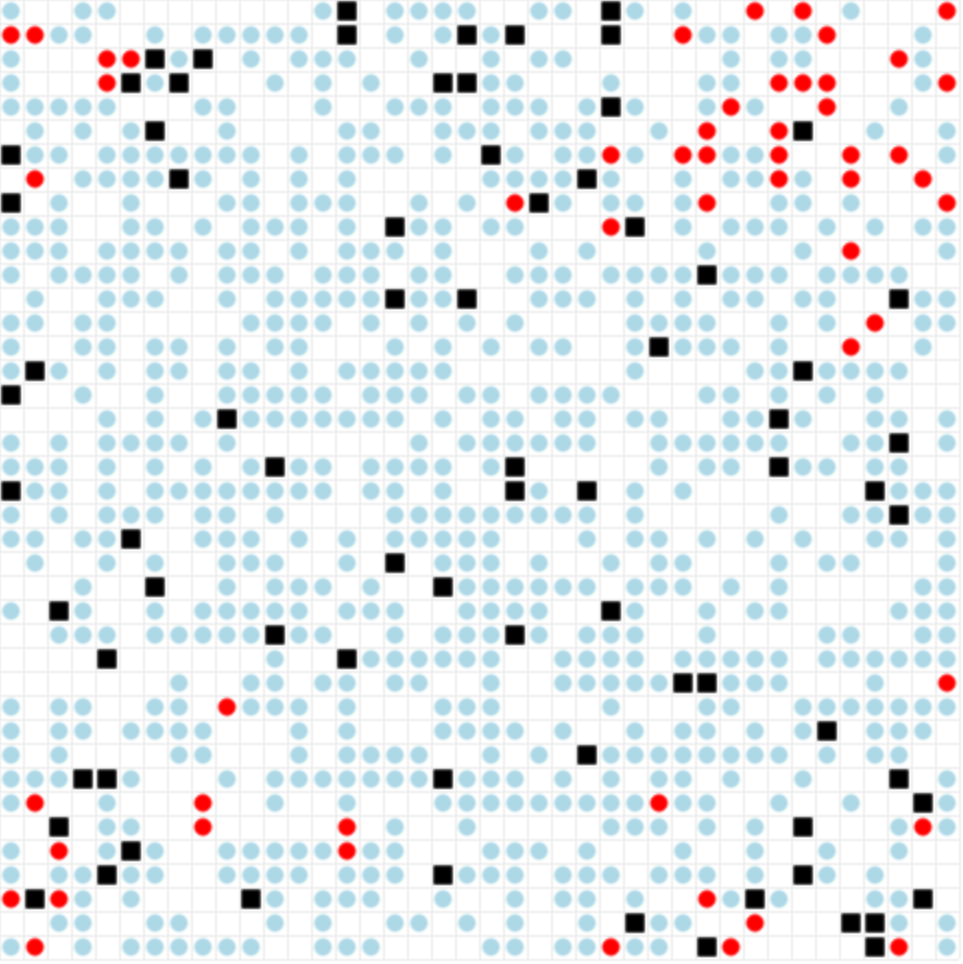
\includegraphics[width=.9\textwidth]{pictures/demonstration/spread_2.png}
                \end{figure}
            \end{column}
            \begin{column}{.3\textwidth}
                \begin{figure}
                    \centering
                    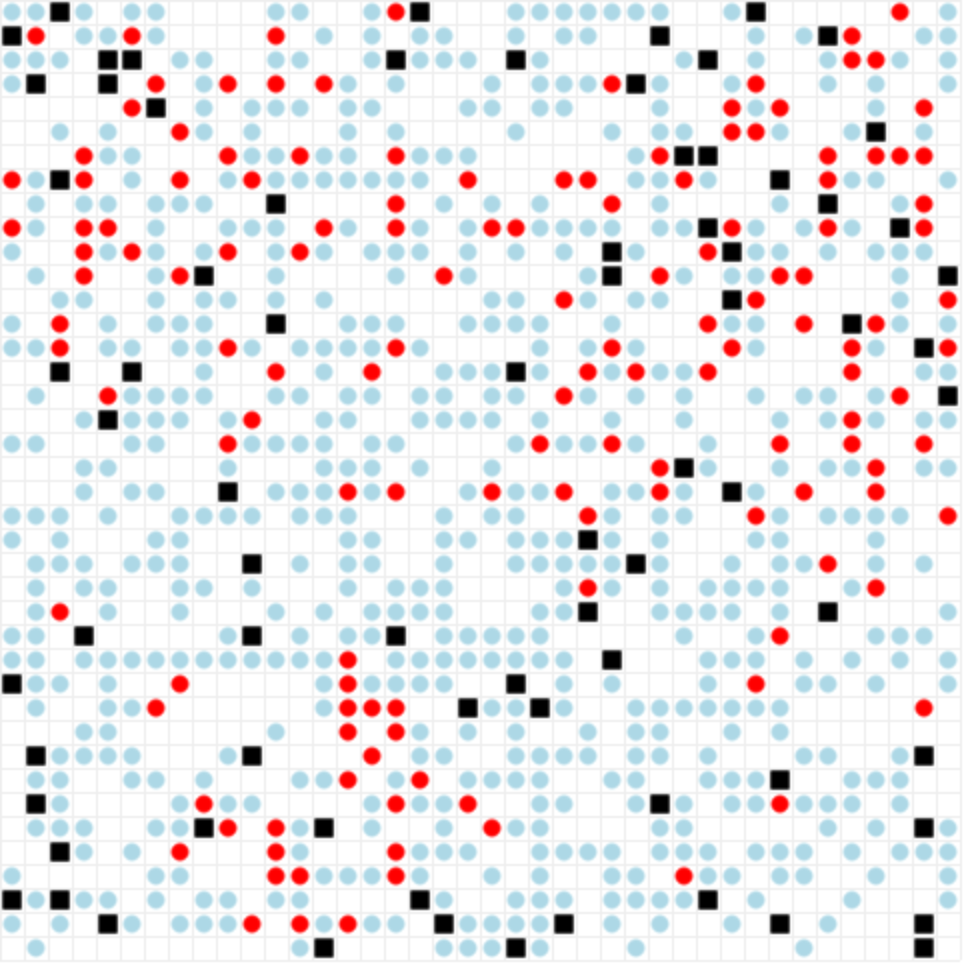
\includegraphics[width=.9\textwidth]{pictures/demonstration/spread_3.png}
                \end{figure}
            \end{column}
        \end{columns}

    \end{frame}

    \section{Sensitivity analysis}

    \begin{frame}{OFAT analysis}

        \begin{columns}
            \begin{column}{0.4\textwidth}
                \begin{itemize}
                    \item Active threshold =  $0.1$
                    \item Initial legitimacy =  $0.8$
                    \item Max jail term = $[30, \infty]$
                    \item Citizen vision  $[1.7,  14]$
                    \item Cop vision = $[1.7, 14]$
                \end{itemize}

                Based on publications from Epstein, Fonoberova, Huang \& Lemos
            \end{column}

            \begin{column}{0.6\textwidth}
                \begin{figure}
                    \centering
                    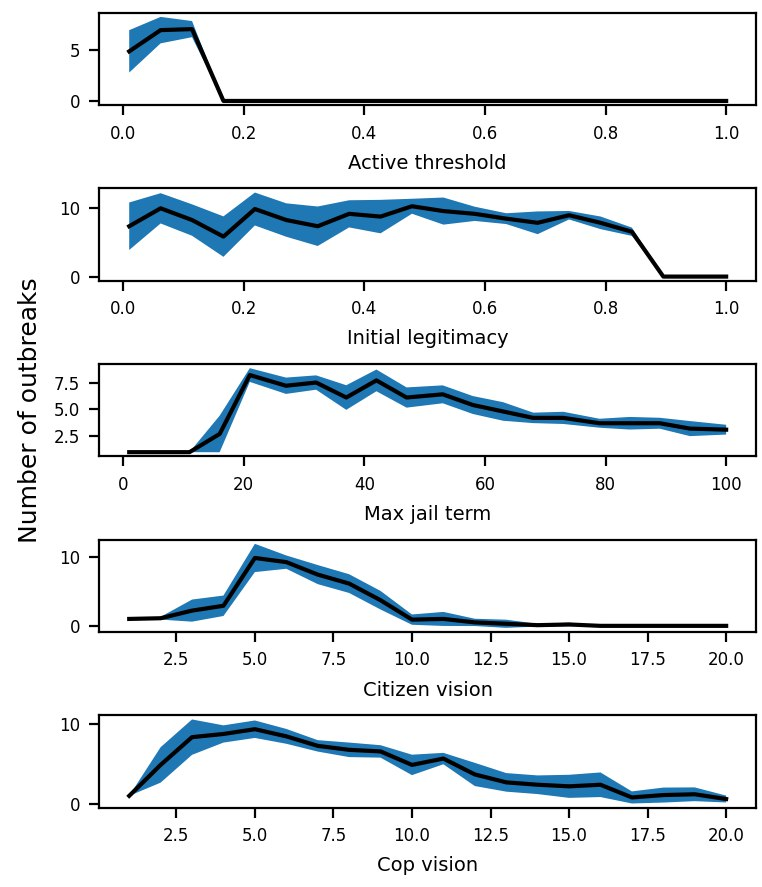
\includegraphics[width=.8\textwidth]{pictures/sensitivity_analysis/ofat-outbreaks.jpg}
                \end{figure}
            \end{column}
        \end{columns}

    \end{frame}


    \begin{frame}{Global analysis}

        \begin{columns}
            \begin{column}{.3\textwidth}
                \begin{itemize}
                    \item All three parameters influence the model
                \end{itemize}
            \end{column}
            \begin{column}{0.7\textwidth}
                \begin{figure}
                    \centering
                    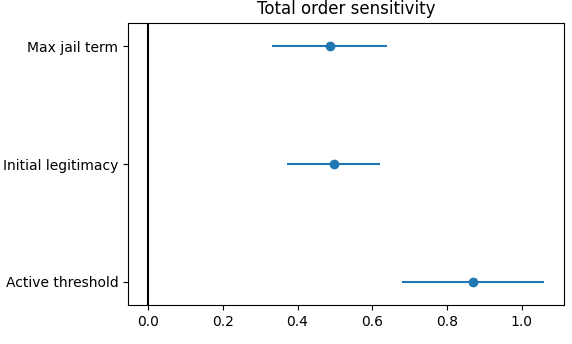
\includegraphics[width=\textwidth]{pictures/sensitivity_analysis/global_sa.png}
                    \caption{Sobol - outbreaks}
                \end{figure}
            \end{column}
        \end{columns}

    \end{frame}


    \section{Results}

    \begin{frame}{Experiment 1 - Influence of network on civil violence}
        \large Effect of network structure on outbreak duration
        \begin{columns}
            \begin{column}{.4\textwidth}
                \begin{itemize}
                    \item No network leads to frequent short outbreaks
                    \item Very similar results for all Network types
                    \begin{itemize}
                        \item Slightly denser around average duration for Albert-Barabasi
                    \end{itemize}
                \end{itemize}
            \end{column}
            \begin{column}{.6\textwidth}
                \begin{figure}
                    \centering
                    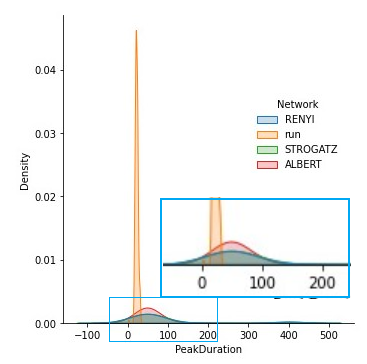
\includegraphics[width=.9\textwidth]{pictures/network_comparison/duration_comparison.png}
                \end{figure}
            \end{column}
        \end{columns}
    \end{frame}

    \begin{frame}{Experiment 1 - Influence of network on civil violence}
        \large Effect of network structure on outbreak sizes
        \begin{columns}
            \begin{column}{.4\textwidth}
                \begin{itemize}
                    \item No network results in smaller outbreaks
                    \item A network structure increases duration and size of outbreaks
                \end{itemize}
            \end{column}
            \begin{column}{.6\textwidth}
                \begin{figure}
                    \centering
                    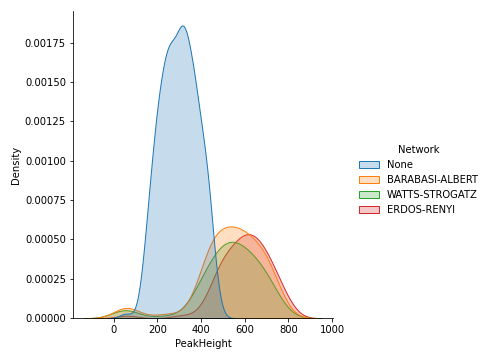
\includegraphics[width=.9\textwidth]{pictures/network_comparison/WithoutRemoveInfluencerDensity.png}
                \end{figure}
            \end{column}
        \end{columns}
    \end{frame}


    \begin{frame}{Experiment 2 - Removing an \textit{influencer} from the model}
        Jailing all influencers at the start of an outbreak.
        \begin{columns}
            \begin{column}{0.3\textwidth}
                \begin{itemize}
                    \item Significant decrease in outbreak size
                    \item More extreme outliers
                \end{itemize}
            \end{column}
            \begin{column}{0.7\textwidth}
                \begin{figure}
                    \centering
                    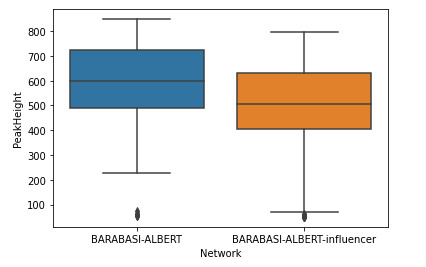
\includegraphics[scale=0.5]{pictures/network_comparison/influencer_removal.jpg}
                \end{figure}

            \end{column}
        \end{columns}
        Effective method for crowd control - similar to (Dutch) riot police
    \end{frame}

    \begin{frame}{Experiment 2 - Removing an \textit{influencer} from the model}
        Jailing all influencers at the start of an outbreak.
        \begin{columns}
            \begin{column}{0.3\textwidth}
                \begin{itemize}
                    \item Significant decrease in outbreak size
                    \item More extreme outliers
                \end{itemize}
            \end{column}
            \begin{column}{0.7\textwidth}
                \begin{figure}
                    \centering
                    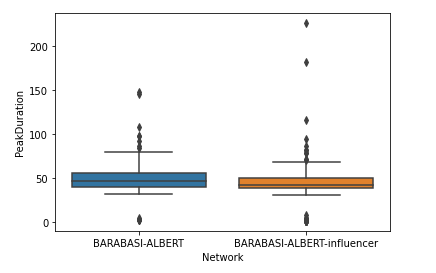
\includegraphics[scale=0.5]{pictures/network_comparison/influencer_removal_duration.jpg}
                \end{figure}

            \end{column}
        \end{columns}
        Effective method for crowd control - similar to (Dutch) riot police
    \end{frame}



    \begin{frame}{Experiment 2 - Removing an \textit{influencer} from the model}
        Jailing all influencers at the start of an outbreak.
        \begin{columns}
            \begin{column}{0.3\textwidth}
                \begin{itemize}
                    \item Significant decrease in outbreak size
                    \item More extreme outliers
                    \item Bimodal distribution
                    \begin{itemize}
                        \item Small peak at outbreak threshold
                    \end{itemize}
                \end{itemize}
            \end{column}
            \begin{column}{0.7\textwidth}
                \begin{figure}
                    \centering
                    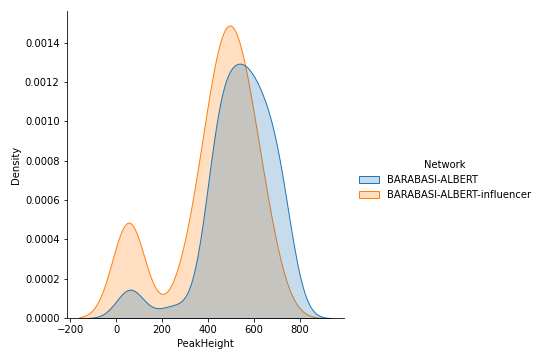
\includegraphics[scale=0.4]{pictures/network_comparison/only2density.png}
                \end{figure}
            \end{column}
        \end{columns}
        Effective method for crowd control - similar to (Dutch) riot police
    \end{frame}

    \section{Conclusion}

    \begin{frame}{Future Work}

        \textbf{We determined that}:
        \begin{itemize}
            \item Social networks contribute to greater propagation and duration of civil violence
            \item Removal of influencer agents might help to mitigate violences.
        \end{itemize}

        \hfill{}

        \textbf{What could be done} ?
        \begin{itemize}
            \item Adjust \emph{Contagious Hardship} equation to reproduce a more realistic transmission of information: \\ Average \emph{civilian} agent hardship should not weight as much as an {influencer} agent hardship
        \end{itemize}

    \end{frame}

    \begin{frame}


        \Huge Questions ?

    \end{frame}

\end{document}